\documentclass[../differential_geometry.tex]{subfiles}
\begin{document}
\section{Aula 21 - 16 de Junho, 2026}
\subsection{Motivações}
\begin{itemize}
	\item Propriedades Minimizantes de Geodésicas;
	\item Geodésicas em Superfícies de Revolução.
\end{itemize}
\subsection{Propriedades Minimizantes de Geodésicas}
Previamente, vimos as equações das geodésicas parametrizada como uma curva \(\beta (t) = \underline{x}(u(t), v(t))\):
\begin{align*}
	 & \boxed{u''E + v''F + \frac{1}{2}(u')^{2}E_{u} + u'v'E_{v}+(v')^{2}\biggl(F_{v}-\frac{1}{2}G_{u}\biggr)=0} \\
	 & \boxed{u''F + v''G + \frac{1}{2}(v')^{2}G_{v} + u'v'G_{u}+(u')^{2}\biggl(F_{u}-\frac{1}{2}E_{v}\biggr)=0}
\end{align*}
Note que as equações dependem apenas dos coeficientes da primeira forma fundamental, que se traduz ao fato das geodésicas serem um conceito intrínseco e dependerem apenas da métrica em S, não do local onde S mora!
\begin{example}[Geodésicas num Plano]
	Espera-se que sejam as geodésicas que conhecemos; tome \(\beta \) uma geodésia, de forma que \(\beta ''\) é ortogonal ao plano, ou seja, sua aceleração é paralela ao plano. Logo, para ser simultaneamente ortogonal e paralela ao plano, \(\beta''\equiv 0 \) e \(\beta '(t) = 0\), dando a forma \(\beta (t) = a + bt\); noutras palavras, \(\beta \) é um segmento de reta!
\end{example}
\begin{example}[Geodésicas num Cilindro]
	Sabemos que, se \(S: x^{2} + y^{2} = r^{2}\) for um cilindro, então
	\[
		f(u, v) = \biggl(r \cos^{}{\frac{u}{r}}, r\sin^{}{\frac{u}{r}}, v\biggr)
	\]
	é uma isometria local entre o plano e o cilindro. Portanto, as geodésicas no cilindro são imagens de retas do plano após passarem por f.
	\begin{figure}[H]
		\begin{center}
			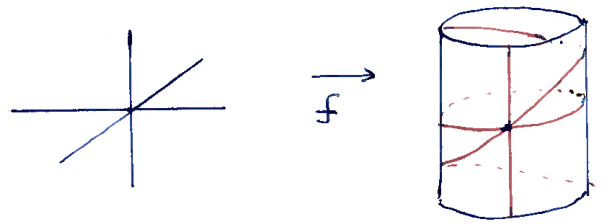
\includegraphics[height=\textheight, width=\textwidth, keepaspectratio]{./Images/cylinder_geodesic_21.png}
		\end{center}
	\end{figure}

	Daí, as três geodésicas possíveis são:
	\begin{align*}
		 & \tikz[baseline=-0.5ex]\draw[black, fill=black, radius=1.5pt](0, 0)circle;\; u_{0} = \mathrm{cte},\; f(u_{0}, v) = \biggl(r\cos^{}{\frac{u_{0}}{r}}, r\sin^{}{\frac{u_{0}}{r}}, v\biggr), v\in \mathbb{R}         \\
		 & \tikz[baseline=-0.5ex]\draw[black, fill=black, radius=1.5pt](0, 0)circle;\; v_{0} = \mathrm{cte},\; f(u, v_{0}) = \biggl(r\cos^{}{\frac{u}{r}}, r\sin^{}{\frac{u}{r}}, v_{0}\biggr), u\in \mathbb{R}             \\
		 & \tikz[baseline=-0.5ex]\draw[black, fill=black, radius=1.5pt](0, 0)circle;\; v=\lambda u+\varphi ,\; f(u, \lambda u+\varphi ) = \biggl(r\cos^{}{\frac{u}{r}}, r\sin^{}{\frac{u}{r}}, \lambda u + \varphi \biggr),
	\end{align*}
	tal que a primeira forma uma geodésica, a segunda um círculo no cilindro, e a última uma hélice.
\end{example}

As geodésicas são muito importantes por serem curvas que minimizam distâncias! No espaço \(\mathbb{R}^{3}\), o caminho mais curto entre dois pontos é o segmento da reta que liga os pontos, mas se considerássemos uma esfera e tentássemos ligar dois pontos em partes opostos (antipodais), o caminho mais rápido seria furando o centro dela! Isso infelizmente não dá, é preciso caminhar pela superfície e minimizar \textit{esse caminho}\footnote{E evitar as guerras.}, resultando em um círculo grande!
\begin{figure}[H]
	\begin{center}
		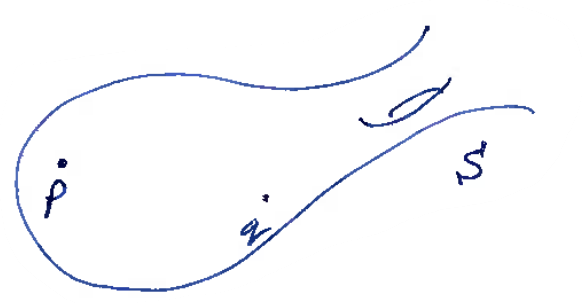
\includegraphics[height=0.6\textheight, width=0.6\textwidth, keepaspectratio]{./Images/points_in_surface_22.png}
	\end{center}
\end{figure}

Suponha que p e q são dois pontos de uma superfície; em geral, o segmento da reta \(pq\) não é um caminho da superfície (o segmento de reta entre SP e Tokyo fura a Terra), e, por isso, buscamos o menor comprimento de uma curva que está na superfície:
\[
	\min\limits_{\gamma }\int_{0}^{1}\Vert \gamma '(t) \Vert \mathrm{d}t, \quad \gamma (0) =p,\; \gamma (1) = q,\; \gamma (t)\in S \; \forall t\in [0, 1]
\]
\begin{tcolorbox}[
		skin=enhanced,
		title=Observação,
		fonttitle=\bfseries,
		colframe=black,
		colbacktitle=cyan!75!white,
		colback=cyan!15,
		colbacklower=black,
		coltitle=black,
		drop fuzzy shadow,
		%drop large lifted shadow
	]
	Um resultado do cálculo variacional, fornecendo os pontos críticos do funcional, é que todas as curvas minimizantes sã geodésicas; porém, \textbf{nem toda geodésica é minimizante!} Basta considerar o exemplo de dois pontos não antipodais um perto do outro, e vai ter uma geodésica minimizante e outra não minimizante.
	\begin{figure}[H]
		\begin{center}
			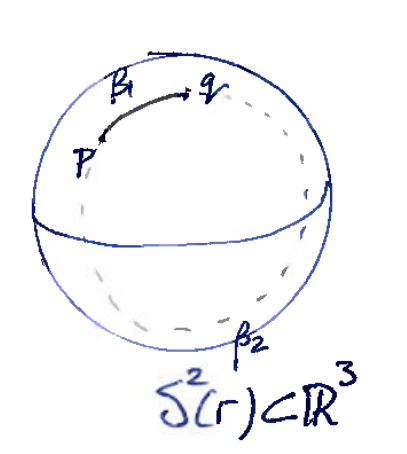
\includegraphics[height=0.5\textheight, width=0.5\textwidth, keepaspectratio]{./Images/nonminimizing_geodesic_22.png}
		\end{center}
	\end{figure}
\end{tcolorbox}

São poucas as superfícies onde podemos caracterizar todas as geodésicas, e veremos algumas delas, incluindo no plano hiperbólico.
\subsection{Geodésicas em Superfícies de Revolução e no Plano Hiperbólico}
Seja \(\underline{x}(u, v)=(f(v)\cos^{}{u}, f(v)\sin^{}{u}, g(v))\) uma parametrização de uma superfície de revolução; temos, então, os coeficientes
\[
	E = f(v)^{2}, \quad F = 0, \quad G = f'(v)^{2} + g'(v)^{2},
\]
tal que a primeira equação das geodésicas vira
\[
	u''E + u'v'E_v = 0 \Longleftrightarrow (u'E)'=0 \quad ((u'E(u, v)'=u''E + [\underbrace{u'E_u}_{\mathclap{0}} + v'E_v)];
\]
logo,
\[
	u'E = \mathrm{cte}.
\]
Vamos provar que todos os meridianos são geodésicas para superfícies de revolução.
\begin{lemma*}
	Todos os meridianos são geodésicas quando parametrizados por comprimento de arco.
\end{lemma*}
\begin{proof*}
	Com a parametrização do enunciado e a equação da geodésica já elaborada, seja \(\beta (t) = (u_{0}(t), v(t))\) um meridiano; precisamos calcular o valor de \(\Vert \beta ' \Vert\) para parametrizá-lo por comprimento de arco:
	\[
		\Vert \beta '(t) \Vert=\Vert v'\underline{x}_v \Vert = \mathrm{cte} \Longleftrightarrow v'^{2}G = k,
	\]
	onde k é constante. Vamos verificar se a \(\beta \) com estas condições satisfaz as equações A e B.

	Com efeito, a primeira equação já foi mostrada ser equivalente a pedir que \(u'E\) seja constante, e como \(u(t) = u_{0}\), temos \(u'(t) = 0\), que satisfaz automaticamente a condição. Por outro lado, para a equação B, segue que
	\[
		v''G + \frac{1}{2}(v')^{2}G_v = 0,
	\]
	mas
	\[
		(v')^{2}G = k \Rightarrow 2v''v'G + (v')^{3}G_v = 0 \Longleftrightarrow v'\biggl(v''G + \frac{1}{2}(v')^{2}G_v\biggr) = 0.
	\]
	Como \(v'\neq 0,\) temos
	\[
		v''G + \frac{1}{2}(v')^{2}G_v = 0,
	\]
	ou seja, B é satisfeita. Portanto, todo meridiano é uma geodésica (numa superfície de revolução). \qedsymbol
\end{proof*}
\begin{lemma*}
	A paralela pelo ponto \((f(v_{0}), 0, g(v_{0}))\), quando parametrizada pelo comprimento de arco, é uma geodésica se, e somente se, \(f'(v_{0}) = 0\).
\end{lemma*}
\begin{proof*}
	Seja \(\beta (t) = \underline{x}(u(t), v_{0})\), tal que
	\[
		\beta '(t) = u'\underline{x}_u \quad\&\quad \beta '';
	\]
	então,
	\[
		\Vert \beta '(t) \Vert=\Vert u'\underline{x}_u \Vert = \mathrm{cte} \Longleftrightarrow (u')^{2}E = k,
	\]
	k constante.

	Porém,
	\[
		E(u(t),v_{0}) = f(v_{0})^{2} = \mathrm{cte},
	\]
	tal que
	\[
		\Vert \beta ' \Vert = \mathrm{cte}\Longleftrightarrow u'=\mathrm{cte},
	\]
	e se \(u'\) e E são constantes, a primeira equação da geodésica é satisfeita.

	Por outro lado, a equação B é satisfeita se, e somente se, \(E_v = 0\), que equivale a \(E_v(v_{0}) = 0\) e
	\[
		E_v(v_{0}) = 0 \Longleftrightarrow 2f(v_{0})f'(v_{0}) = 0 \Longleftrightarrow f'(v_{0})=0,
	\]
	provando o resultado. \qedsymbol
\end{proof*}

E as outras geodésicas? Como se comportam?
\begin{theorem*}[Teorema da Relação de Clairaut]
	Para uma geodésica qualquer \(\beta (t) = \underline{x}(u(t), v(t))\) numa superfície de revolução S, se \(\theta (t)\) é o ângulo que ela faz com as paralelas pelo ponto \(\beta (t)\), então
	\[
		f(v(t))\cos^{}{\theta (t)}=c
	\]
	para alguma constante c.
\end{theorem*}
\begin{figure}[H]
	\begin{center}
		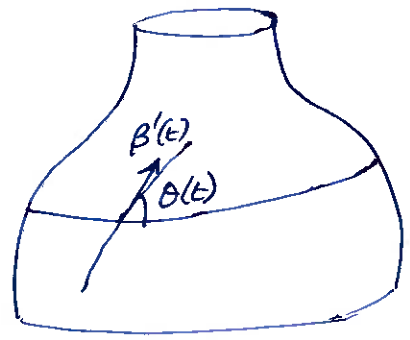
\includegraphics[height=0.4\textheight, width=0.4\textwidth, keepaspectratio]{./Images/clairaut_relationship_22.png}
	\end{center}
\end{figure}
\begin{proof*}
	Por definição,
	\begin{align*}
		\cos^{}{\theta (t)} = \frac{\langle \underline{x}_{u}, \beta ' \rangle}{\Vert \underline{x}_u \Vert \Vert \beta' \Vert} & = \frac{\langle \underline{x}_{u}, u'\underline{x}_{u} + v; \underline{x}_{v} \rangle}{\sqrt[]{E}\Vert \beta ' \Vert} \\
		                                                                                                                        & = \frac{u'E}{\sqrt[]{E}\Vert \beta ' \Vert}                                                                           \\
		                                                                                                                        & = \frac{u'\sqrt[]{E}}{\Vert \beta ' \Vert},
	\end{align*}
	logo, pela equação A,
	\[
		\sqrt[]{E}\cos^{}{\theta (t)}=\frac{u'E}{\Vert \beta '\Vert} = \mathrm{cte}.
	\]
	Portanto, como \(E = f(v)^{2}\), temos
	\[
		f(v(t))\cos^{}{\theta (t)}=c.\text{ \qedsymbol}
	\]
\end{proof*}
\end{document}

